\PassOptionsToPackage{subsection=false}{beamerouterthememiniframes}
\documentclass{beamer}

\usetheme{Szeged}
%\usepackage{pgfpages}
%\setbeameroption{show notes on second screen=right}
\setbeamertemplate{navigation symbols}{}
%\usecolortheme[named=black]{structure}
\definecolor{db}{HTML}{3A4454}
\definecolor{elblue}{HTML}{53687e}
\setbeamercolor{palette primary}{bg=blue,fg=white}
\setbeamercolor{palette secondary}{bg=blue,fg=white}
\setbeamercolor{palette tertiary}{bg=elblue,fg=white}
\setbeamercolor{palette quaternary}{bg=black,fg=white}
\setbeamercolor{structure}{fg=db} % itemize, enumerate, etc
\setbeamercolor{section in toc}{fg=black} % TOC sections
\setbeamercolor{frametitle}{bg=white,fg=elblue}
% Override palette coloring with secondary
\setbeamercolor{subsection in head/foot}{bg=gray,fg=white}

\setbeamertemplate{section in toc}{\inserttocsectionnumber.~\inserttocsection}

\usepackage{xurl}
\usepackage{amsmath,amsfonts}
\usepackage{tikz}
\usetikzlibrary{shapes.geometric, arrows}
\usepackage{mathrsfs}
\usefonttheme[onlymath]{serif}

\newcommand{\R}{\mathbb{R}}
\newcommand{\E}{\mathbb{E}}
\newcommand\dint{\mathord{\mathrm{d}}}
\newcommand{\M}{\mathbf{M}}
\newcommand{\A}{\mathbf{A}}
\newcommand{\B}{\mathbf{B}}

\begin{document}

\title{Charakteristische Funktionen}
%\subtitle{}
\author{Maximilian Ernst}
\date{\today}
\begin{frame}
\titlepage
\end{frame}

\begin{frame}\frametitle{Inhalt}\tableofcontents\end{frame}

%%%%%%%%%%%%%%%%%%%%%%%%%%%%%%%%%%%%
\section{Motivation}
%%%%%%%%%%%%%%%%%%%%%%%%%%%%%%%%%%%%
\begin{frame}
\frametitle{Dualität}
\textit{Manchmal bilden sehr unterschiedliche mathematische Objekte nur zwei Seiten der selben Medaille}

\hfill \newline
\hfill \newline

Ziel: Jeder (reellwertigen) Zufallsvariable ein möglichst "einfaches" mathematisches "Objekt" zuordnen, sodass wir Berechnungen und Beweise mit diesem Objekt (statt der Zufallsvariable) machen.
\end{frame}

\begin{frame}
\frametitle{Ziel}
\begin{itemize}
    \setlength\itemsep{1em}
    \item[--] Verteilung der Summe unabhängiger Zufallsvariablen
    \item[--] Berechnung von Momenten
    \item[--] Beweis von Verteilungskonvergenzen
\end{itemize}
\end{frame}

\begin{frame}
\frametitle{Beispiel 1}
Betrachte die Menge aller Kreise.

Die duale Menge ist die Menge alle einbeschriebenen Quadrate.
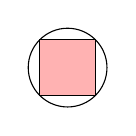
\begin{tikzpicture}
\node (start) [circle, minimum width=1cm, minimum height=1cm, text centered, draw=black] {};
\node (end) [rectangle, minimum width=0.7061cm, minimum height=0.7061cm, text centered, draw=black, fill=red!30] {};
\end{tikzpicture}

Die Relation $>$ für den Flächeninhalt bleibt erhalten. Wollen wir also wissen, ob ein Kreis größer als ein anderer ist, können wir stattdessen auch schauen, ob das einbeschriebene Quadrat größer ist.
\end{frame}

\begin{frame}
\frametitle{Beispiel 2}
Logarithmieren zur Berechnung von Produkten.

Die Menge sind die positiven reellen Zahlen, und die duale Menge sind auch die positiven reellen Zahlen.

Die strukturerhaltende Abbildung ist der Logarithmus; die Multiplikation von reellen Zahlen entspricht der Addition:

$$\ln xy = \ln x + \ln y $$

Zur Berechnung großer Produkte:
Berechne den Logarithmus; addiere das Ergebnis; nimm $\exp$ des Ergebnisses.

\end{frame}

\begin{frame}
\frametitle{Beispiel 3}
Es gilt (bei fester Basis): jeder linearen Funktionen $f: \R^n \to \R^n$ kann eineindeutig eine Matrix zugeordnet werden, die sogennante Darstellungsmatrix $\M_f$, sodass gilt:

$$f(x) = \M_fx$$

Die erhalten bleibende Struktur ist die Verknüpfung von Funktionen:

$$\M_{f \circ g} = \M_f \M_g$$

Außerdem gilt:

$$f \; \text{ist bijektiv} \iff \M_f \; \text{ist invertierbar}$$
\end{frame}

\begin{frame}
\frametitle{Ein einfacher Beweis}
$\A, \B \in \R^{n \times n}$ sind invertierbar $\implies \A \B$ ist invertierbar
\hfill \break
\hfill \break
Beweis:
\begin{enumerate}
  \item \textbf{Gehe in die duale Menge:} \hfill \break
  Es existieren lineare Funktionen $f, g: \R^n \to \R^n$ sodass
  \begin{itemize}
    \item[--] $\A$ die Darstellungsmatrix von $f$ ist
    \item[--] $\B$ die Darstellungsmatrix von $g$ ist
    \item[--] $f, g$ sind bijektiv
  \end{itemize}
  \item \textbf{Führe den Beweis in der dualen Struktur:} \hfill \break
  Da $f, g$ bijektiv sind, ist auch $f \circ g$ bijektiv.
  \item \textbf{Gehe zurück in die ursrüngliche Menge:} \hfill \break
    Es ist dann $\A \B$ die Darstellungsmatrix von $f \circ g$, und da $f \circ g$ bijektiv ist, ist $\A \B$ invertierbar.
\end{enumerate}

\end{frame}

%%%%%%%%%%%%%%%%%%%%%%%%%%%%%%%%%%%%
\section{Definition}
%%%%%%%%%%%%%%%%%%%%%%%%%%%%%%%%%%%%

\begin{frame}
\frametitle{Mittel}
Wir bestimmen eine (strukturerhaltende) bijektive Abbildung aus der Menge aller reellwertigen Zufallsvariablen in einen andere Menge.

Dann zeigen wir, dass wir anstelle mit den Zufallsvariablen zu rechnen, auch viel einfacher mit ihrem "Partner" rechnen können.
\end{frame}

\begin{frame}
\frametitle{Definition}
Für eine Zufallsvariable X mit Werten in $\R$ bezeichnet
\begin{align} \label{eq1}
\varphi^X(u) &= \E[e^{iuX}] \\
 & = \int_{\R} e^{iux} \dint P^X(x)\\
 & = \int_{\R} \cos(ux) \dint P^X(x) + i \int_{\R} \sin(ux) \dint P^X(x)
\end{align}

ihre charakteristische Funktion.

\end{frame}

\begin{frame}
\frametitle{Eigenschaften}
$\varphi$ sollte besonders "einfach" sein
\hfill \newline
\begin{itemize}
    \setlength\itemsep{1em}
    \item[--] $\varphi(0) = 1$
    \item[--] $|\varphi| \leq 1$
    \item[--] gleichmäßig stetig
\end{itemize}
\end{frame}

\begin{frame}
\frametitle{Berechnungsbeispiel + zeigen, dass die Funktion einfach ist}
\end{frame}

%%%%%%%%%%%%%%%%%%%%%%%%%%%%%%%%%%%%
\section{Anwendung}
%%%%%%%%%%%%%%%%%%%%%%%%%%%%%%%%%%%%

\begin{frame}
\frametitle{Faltung - Dichten}
  Seien $X, Y$ unabhängige reellwertige ZV die beide eine Dichte $f^X, f^Y$ besitzen. Dann besitzt $X+Y$ die Dichte

\begin{equation*}
  f^{X+Y}(z) = \int_{\R} f^X(z - y)f^Y(y) \dint y, \; z \in \R
\end{equation*}

(eng.: convolution)
\end{frame}

\begin{frame}
\frametitle{Faltung - CF}
  Seien $X, Y$ unabhängige reellwertige ZV mit charakteristischen Funktionen $\varphi^X, \varphi^Y$. Dann besitzt $X + Y$ die charakteristische Funktion
$$\varphi^{X+Y} = \varphi^X \varphi^Y$$
\end{frame}

\begin{frame}
\frametitle{Faltung - Beispiel}

\end{frame}

\begin{frame}
\frametitle{Momente}
Besitzt die ZV $X \; p$ endliche Momente, ist $\varphi^X \; p$-mal stetig differenzierbar und es gilt für $k < p$

\begin{equation*}
\E[X^k] = \frac{(\varphi^X)^{(k)}(0)}{i}
\end{equation*}
\end{frame}

\begin{frame}
\frametitle{Momente - Beispiel}
\end{frame}

\begin{frame}
\frametitle{Konvergenz in Verteilung}
\textbf{Stetigkeitssatz von Levy:} \hfill \newline
Seien $P_n$ Wahrscheinlichkeitsmaße auf $(\R, \mathfrak{B}_\R)$ mit charakteristischen Funktionen $\varphi_n$ und gilt $\lim_{n \to \infty} \varphi_n (x) = \varphi(x)$ für alle $x \in \R$ und eine bei $x = 0$ stetige Funktion $\varphi$, so ist $\varphi$ die charakteristische Funktion eines Wahrscheinlichkeitsmaßes $P$ auf $(\R, \mathfrak{B}_\R)$ und es gilt: $P_n \to P$.
\end{frame}

\begin{frame}
\frametitle{Konvergenz in Verteilung - Beispiel}
Poissonscher Grenzwertsatz oder ZGWS
\end{frame}

\begin{frame}
\frametitle{}
\end{frame}

\begin{frame}
\frametitle{}
\end{frame}


%%%%%%%%%%%%%%%%%%%%%%%%%%%%%%%%%%%%
\section*{Referenzen}
%%%%%%%%%%%%%%%%%%%%%%%%%%%%%%%%%%%%

\frame{
\frametitle{Links}

}
\end{document}
